\documentclass{article}
\usepackage[utf8]{inputenc}
\usepackage[french]{babel}
\usepackage{graphicx}
\usepackage{listings}
\usepackage{color}
\usepackage{hyperref}
\usepackage{geometry}
\usepackage{titling}
\usepackage{fancyhdr}
\usepackage{xcolor}
\usepackage{sectsty}
\usepackage{setspace}
\geometry{a4paper, margin=2.5cm}

% Configuration des listings pour le code
\definecolor{codegreen}{rgb}{0,0.6,0}
\definecolor{codegray}{rgb}{0.5,0.5,0.5}
\definecolor{codepurple}{rgb}{0.58,0,0.82}
\definecolor{backcolour}{rgb}{0.95,0.95,0.92}
\definecolor{deepblue}{rgb}{0.0, 0.2, 0.5}

\lstdefinestyle{mystyle}{
    backgroundcolor=\color{backcolour},   
    commentstyle=\color{codegreen},
    keywordstyle=\color{magenta},
    numberstyle=\tiny\color{codegray},
    stringstyle=\color{codepurple},
    basicstyle=\ttfamily\footnotesize,
    breakatwhitespace=false,         
    breaklines=true,                 
    captionpos=b,                    
    keepspaces=true,                 
    numbers=left,                    
    numbersep=5pt,                  
    showspaces=false,                
    showstringspaces=false,
    showtabs=false,                  
    tabsize=2
}

\lstset{style=mystyle}

% Personnalisation des titres de section
\sectionfont{\color{deepblue}\large\bfseries}
\subsectionfont{\color{deepblue}\normalsize\bfseries}

% En-têtes et pieds de page
\pagestyle{fancy}
\fancyhf{}
\fancyhead[L]{TP6: Jenkins-Ansible}
\fancyhead[R]{Ahmed Abd Dayem - 23243}
\fancyfoot[C]{\thepage}
\renewcommand{\headrulewidth}{0.4pt}
\renewcommand{\footrulewidth}{0.4pt}

% Personnalisation de la page de titre
\title{\Huge{\textbf{TP 6 : Intégration Jenkins-Ansible}}}
\author{\Large{Ahmed Abd Dayem Ahmed Bouha} \\ \\ \large{Matricule : \textbf{23243}} \\ \vspace{2cm} \large{Matière : \textbf{IRT43: DevOps}}}
\date{\today}

\begin{document}

% Page de titre personnalisée
\begin{titlepage}
    \centering
    \vspace*{1cm}
    
    
\includegraphics[width=0.4\textwidth]{images/jenkins_logo.png}\\[1cm]
    
    \rule{\linewidth}{0.5mm} \\[0.5cm]
    {\Huge\bfseries\color{deepblue} TP 6 : Intégration\\Jenkins-Ansible\par}
    \rule{\linewidth}{0.5mm} \\[1.5cm]
    
    {\LARGE\bfseries Ahmed Abd Dayem Ahmed Bouha\par}
    \vspace{0.5cm}
    {\large Matricule : \textbf{23243}\par}
    \vspace{1.5cm}
    {\large\bfseries Matière : \textbf{IRT43: DevOps}\par}
    \vspace{1.5cm}
    {\large\today\par}
    \vfill
    
    \begin{flushright}
    {\LARGE\bfseries Professeur : Dr. Fatimetou Abdou\par}
    \end{flushright}
    
    \vspace{1cm}
\end{titlepage}

\thispagestyle{empty}
\begin{center}
\Large{\textbf{Table des matières}}
\end{center}
\tableofcontents
\thispagestyle{empty}
\newpage

\setspace{1.1}
\setcounter{page}{1}
\section{Introduction}
Ce rapport présente la réalisation du TP 6 portant sur l'intégration de Jenkins avec Ansible pour automatiser le déploiement d'applications depuis GitHub. Ce projet démontre la mise en place d'un pipeline CI/CD complet qui permet d'extraire du code source depuis un dépôt GitHub et de le déployer automatiquement sur des serveurs cibles à l'aide d'Ansible.

\subsection{Objectifs du TP}
Les principaux objectifs de ce travail pratique sont les suivants :
\begin{itemize}
    \item Configurer Jenkins avec les plugins nécessaires
    \item Créer un pipeline Jenkins qui s'intègre avec GitHub
    \item Automatiser le déploiement d'une application web avec Ansible
    \item Implémenter une solution CI/CD complète
\end{itemize}

\section{Environnement de travail}
\subsection{Configuration système}
\begin{itemize}
    \item Système d'exploitation : Linux 6.12.10-76061203-generic
    \item Shell : /usr/bin/bash
\end{itemize}

\subsection{Outils utilisés}
\begin{itemize}
    \item Jenkins : pour l'orchestration du pipeline CI/CD
    \item Ansible : pour l'automatisation du déploiement
    \item GitHub : pour héberger le code source
    \item Apache : comme serveur web pour l'application déployée
\end{itemize}

\section{Installation et configuration de Jenkins}
\subsection{Installation de Jenkins}
% Étape 1: Installer Jenkins

\begin{figure}[h]
    \centering
    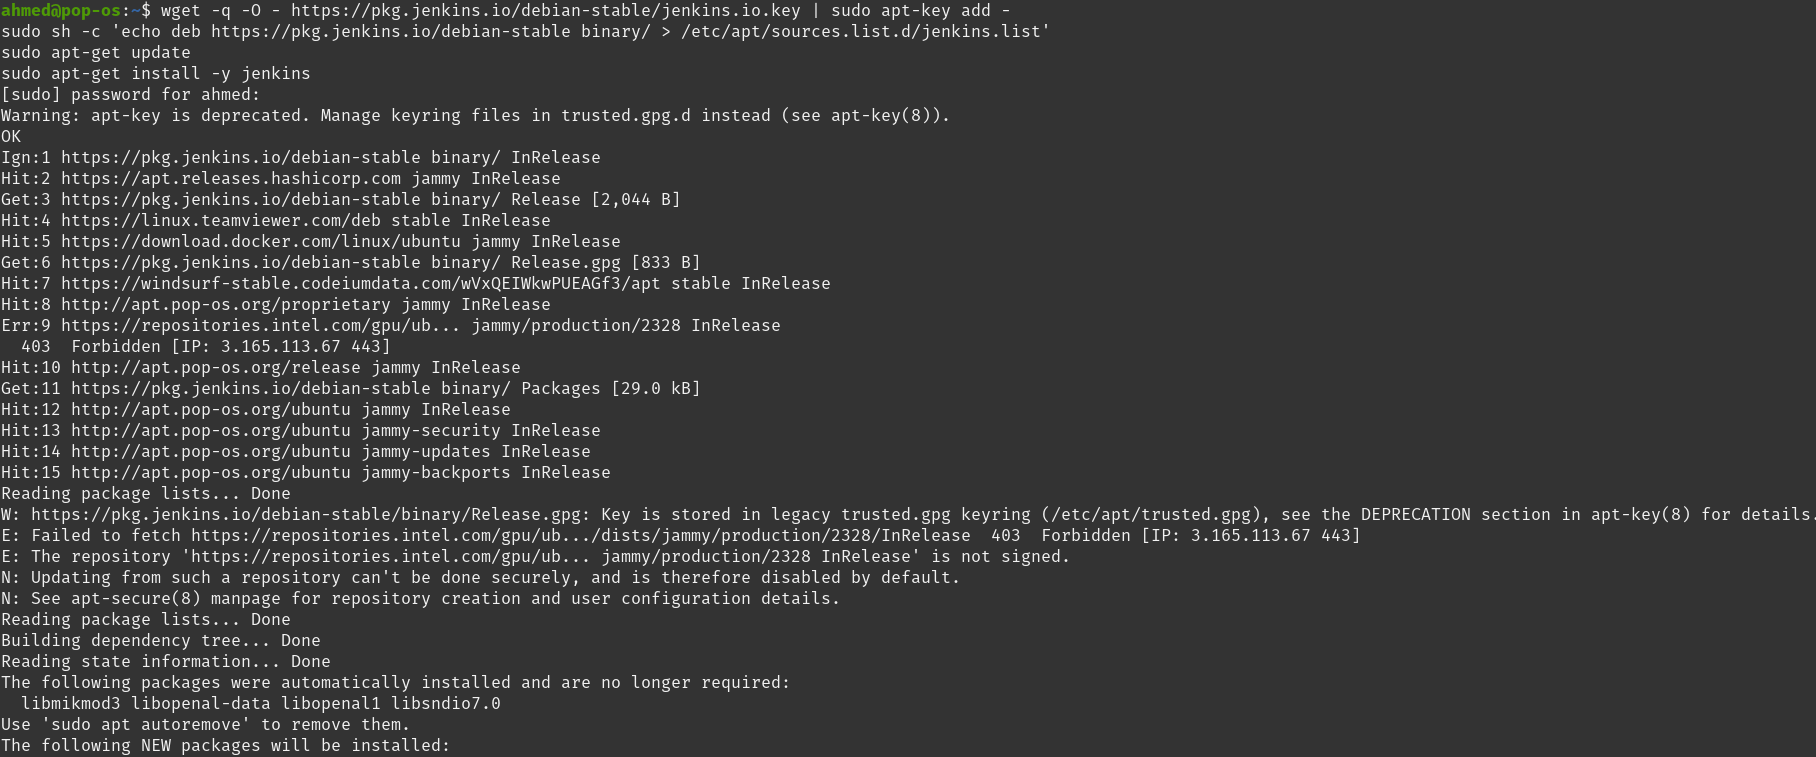
\includegraphics[width=0.8\textwidth]{images/jenkins_installation.png}
    \caption{Installation de Jenkins}
    \label{fig:jenkins_installation}
\end{figure}

J'ai commencé par installer Jenkins en suivant les commandes recommandées :

\begin{lstlisting}[language=bash]
wget -q -O - https://pkg.jenkins.io/debian-stable/jenkins.io.key | sudo apt-key add -
sudo sh -c 'echo deb https://pkg.jenkins.io/debian-stable binary/ > /etc/apt/sources.list.d/jenkins.list'
sudo apt-get update
sudo apt-get install -y jenkins
\end{lstlisting}

Après l'installation, j'ai vérifié que le service Jenkins était bien en cours d'exécution :

\begin{lstlisting}[language=bash]
sudo systemctl status jenkins
\end{lstlisting}

\subsection{Configuration initiale}
Pour la configuration initiale de Jenkins, j'ai récupéré le mot de passe administrateur initial :

\begin{lstlisting}[language=bash]
sudo cat /var/lib/jenkins/secrets/initialAdminPassword
\end{lstlisting}

\begin{figure}[h]
    \centering
    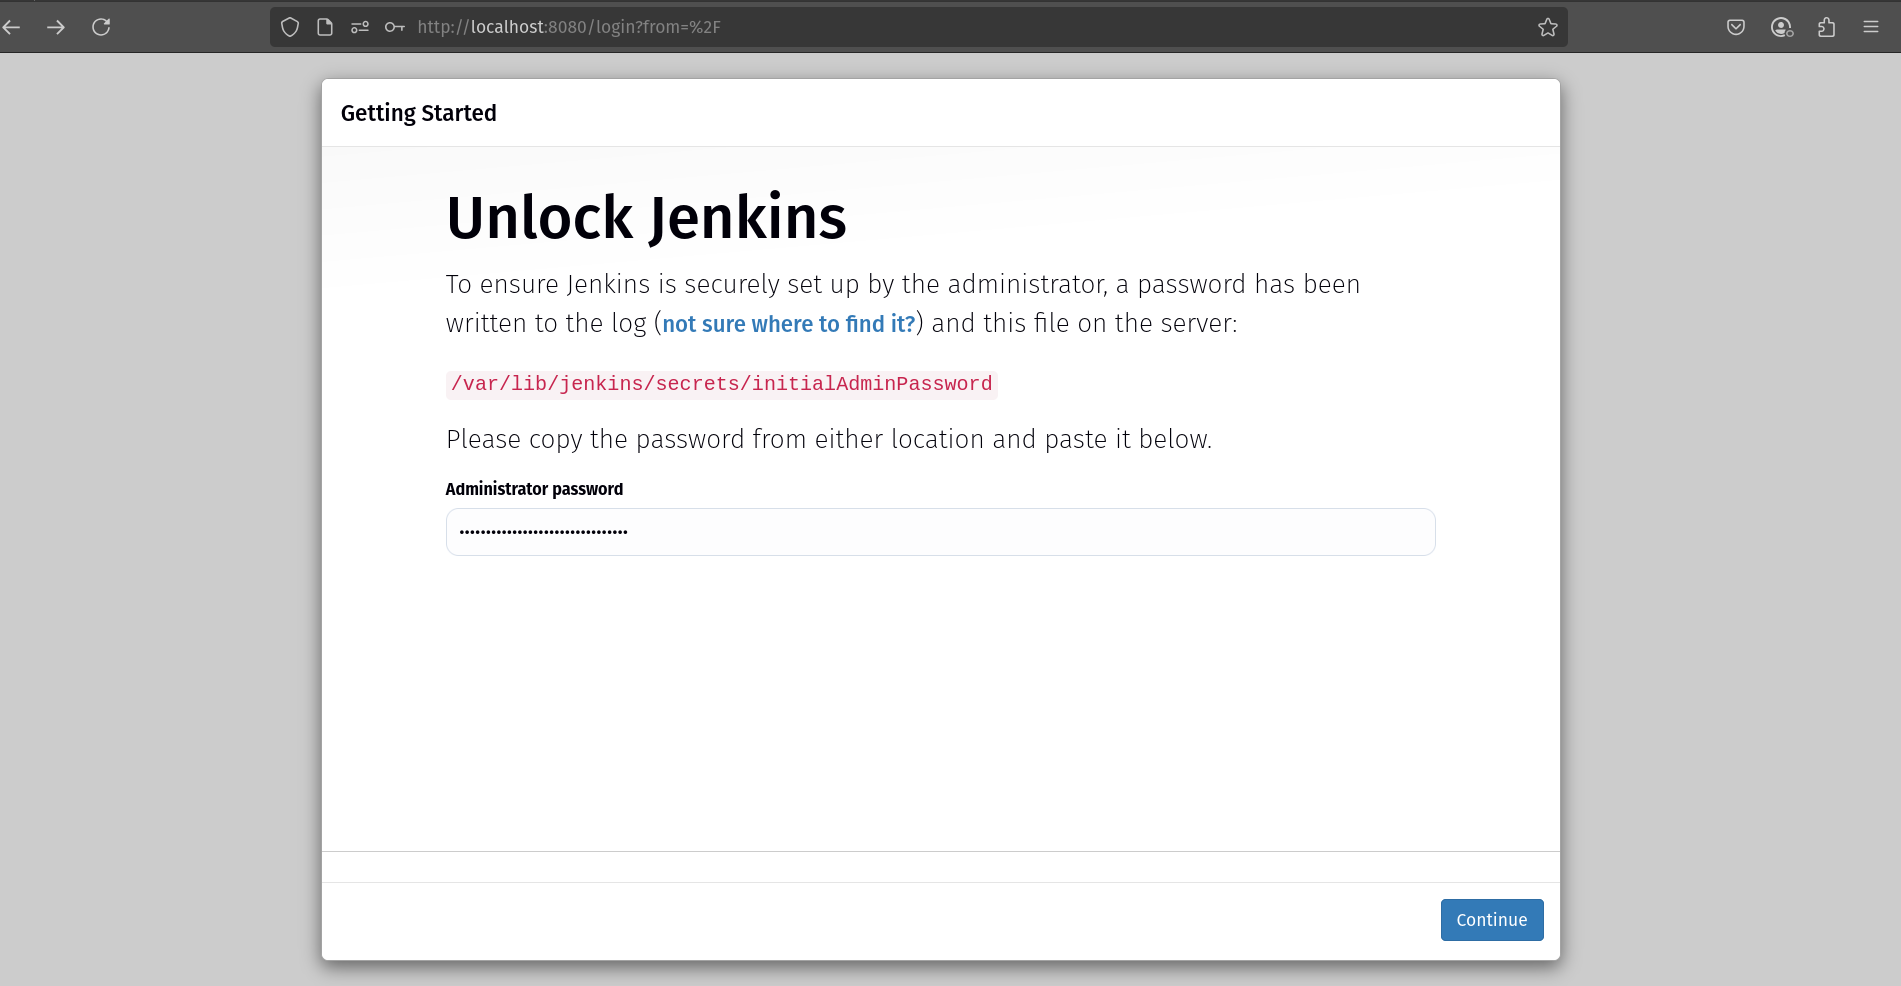
\includegraphics[width=0.8\textwidth]{images/jenkins_unlock.png}
    \caption{Page de déverrouillage Jenkins}
    \label{fig:jenkins_unlock}
\end{figure}

J'ai ensuite suivi l'assistant de configuration pour :
\begin{itemize}
    \item Installer les plugins recommandés
    \item Créer un compte administrateur
    \item Configurer l'URL de Jenkins
\end{itemize}

\begin{figure}[h]
    \centering
    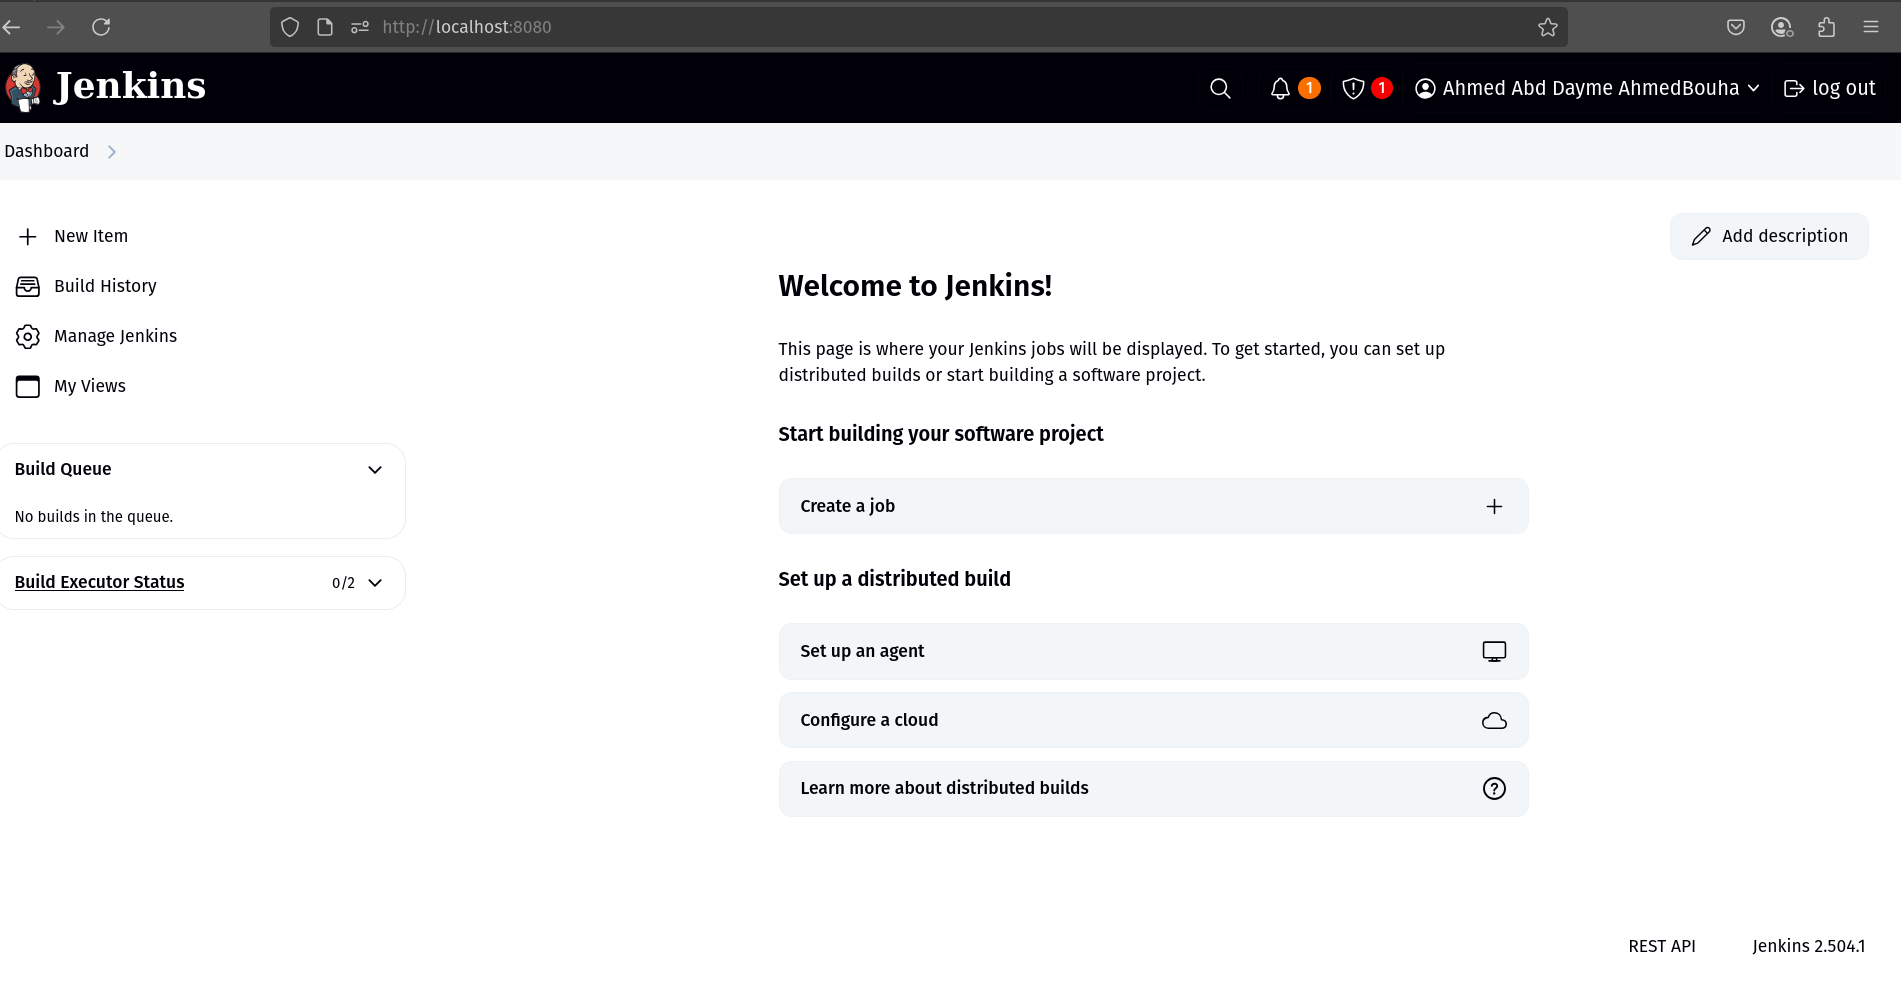
\includegraphics[width=0.8\textwidth]{images/jenkins_dashboard.png}
    \caption{Dashboard Jenkins après configuration}
    \label{fig:jenkins_dashboard}
\end{figure}

\section{Installation des plugins spécifiques}
\subsection{Installation des plugins requis}
Pour ce TP, j'ai installé les plugins suivants depuis l'interface de gestion de plugins de Jenkins (Manage Jenkins > Manage Plugins) :
\begin{itemize}
    \item Git Plugin : pour interagir avec les dépôts Git
    \item GitHub Integration Plugin : pour l'intégration avec GitHub
    \item Ansible Plugin : pour exécuter des playbooks Ansible
\end{itemize}

\begin{figure}[h]
    \centering
    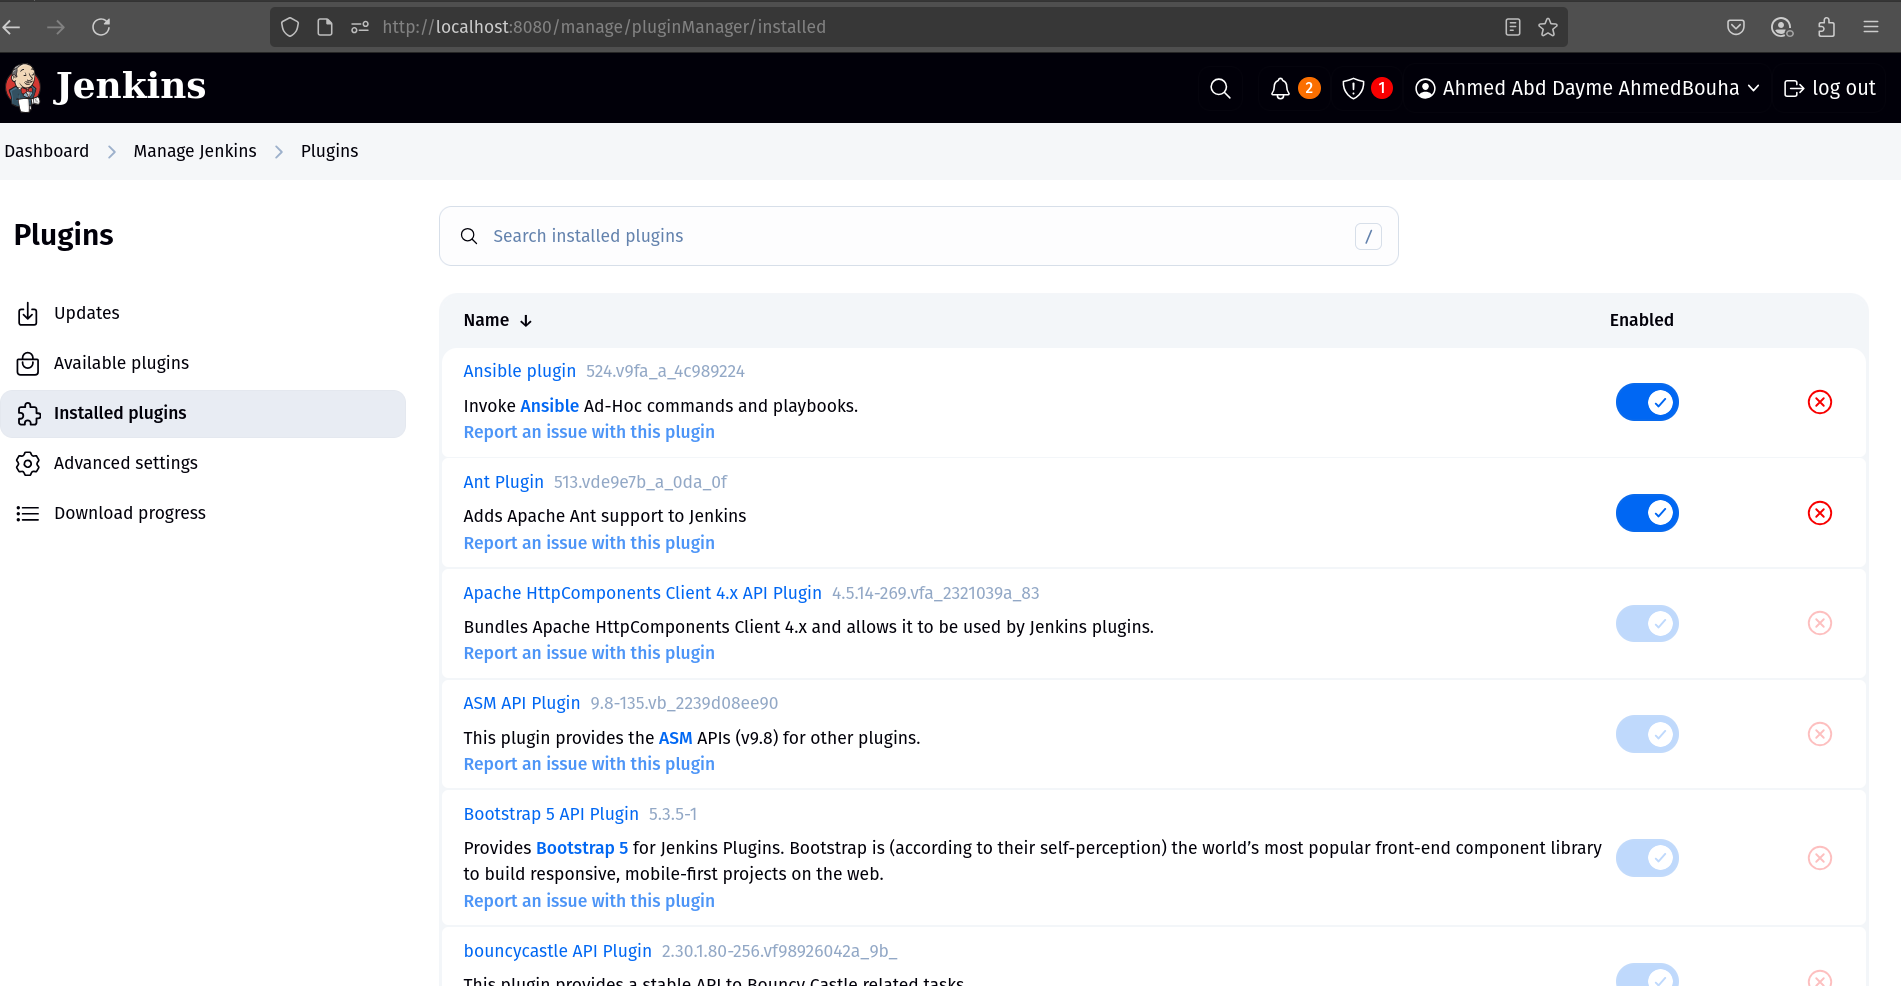
\includegraphics[width=0.8\textwidth]{images/jenkins_plugins.png}
    \caption{Installation des plugins Jenkins}
    \label{fig:jenkins_plugins}
\end{figure}

\section{Préparation du dépôt GitHub}
\subsection{Création et configuration du dépôt}

J'ai créé un dépôt GitHub nommé \texttt{dev\_ansible} pour héberger le code source du projet. Voici les commandes que j'ai utilisées pour initialiser le dépôt :

\begin{lstlisting}[language=bash]
echo "# dev_ansible" >> README.md
git init
git add README.md
git commit -m "first commit"
git branch -M main
git remote add origin git@github.com:ahmedabddayme3752/dev_ansible.git
git push -u origin main
\end{lstlisting}

Ensuite, j'ai ajouté tous les fichiers du projet dans le dépôt :

\begin{lstlisting}[language=bash]
git add .
git commit -m "Add project files"
git push -u origin main
\end{lstlisting}

\begin{figure}[h]
    \centering
    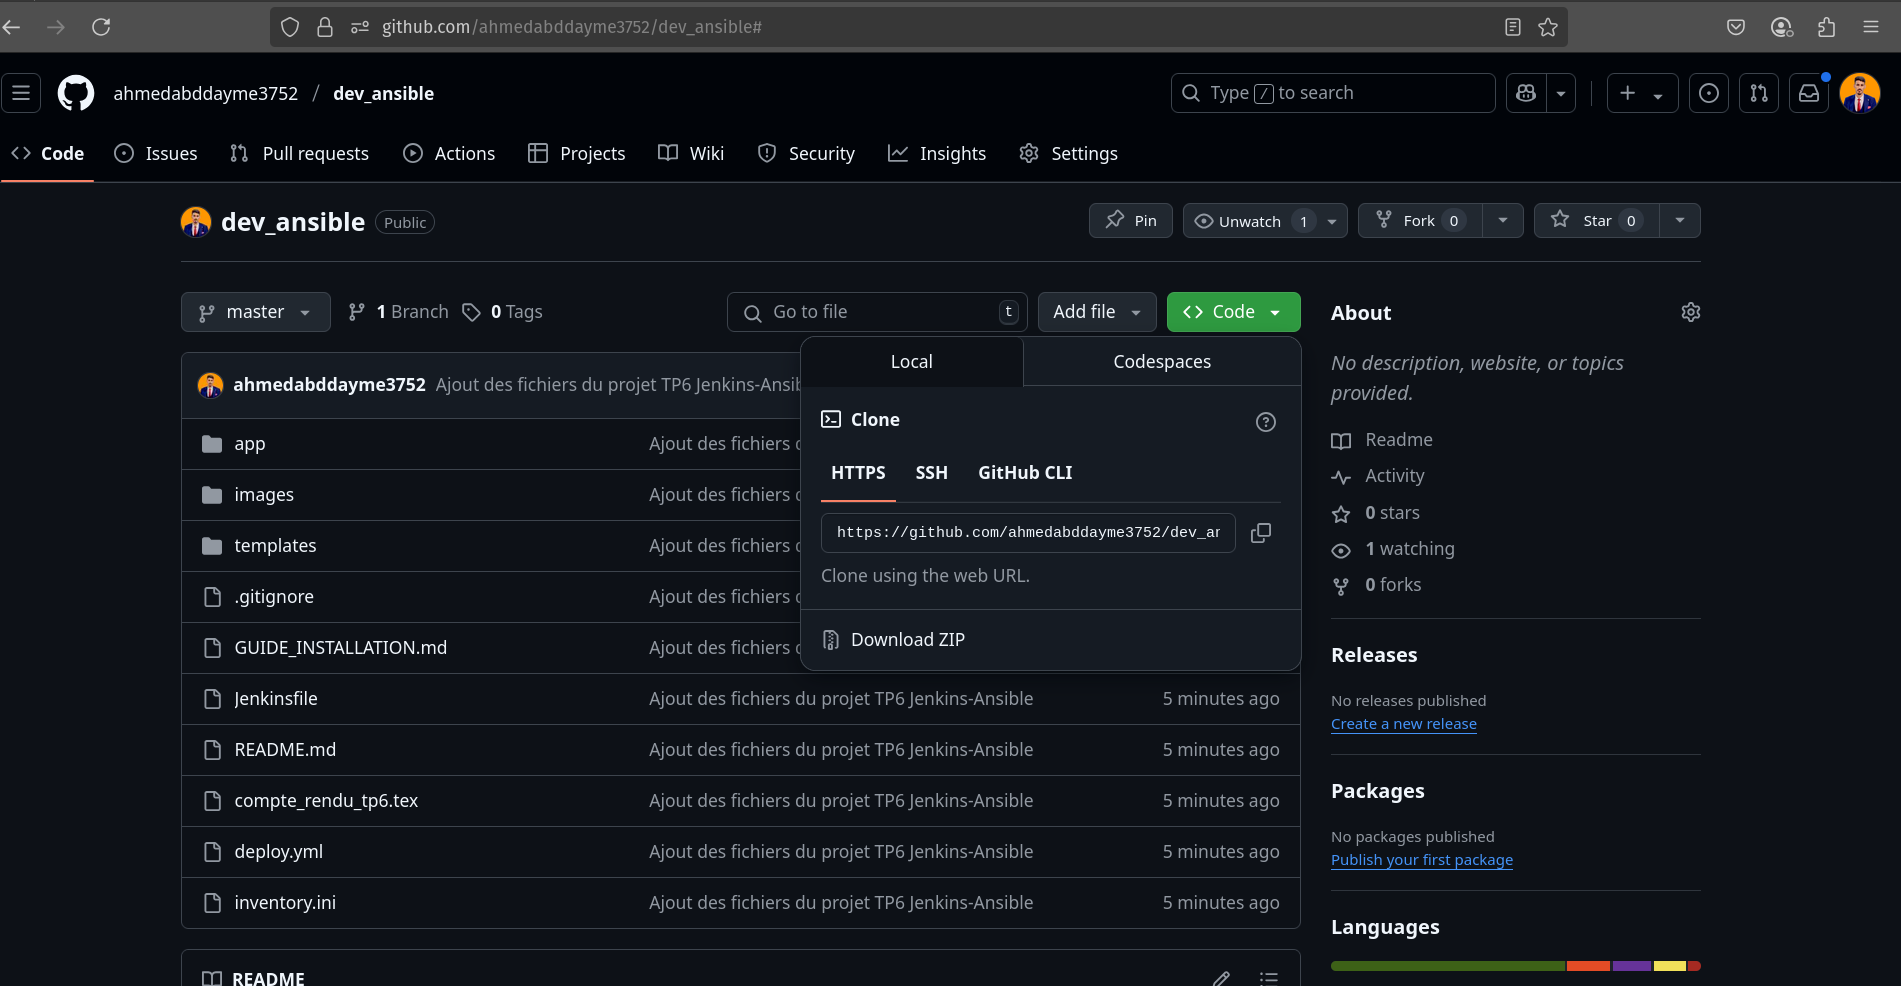
\includegraphics[width=0.8\textwidth]{images/github_repo.png}
    \caption{Dépôt GitHub avec les fichiers du projet}
    \label{fig:github_repo}
\end{figure}

\subsection{Structure du projet}
Le projet contient les fichiers suivants :
\begin{itemize}
    \item \texttt{Jenkinsfile} : Configuration du pipeline CI/CD
    \item \texttt{inventory.ini} : Fichier d'inventaire Ansible définissant les hôtes cibles
    \item \texttt{deploy.yml} : Playbook Ansible pour le déploiement de l'application
    \item \texttt{app/} : Répertoire contenant l'application web à déployer
    \item \texttt{templates/} : Répertoire contenant les templates pour la configuration
\end{itemize}

\section{Création et configuration du pipeline Jenkins}
\subsection{Création du job pipeline}

Pour créer le pipeline Jenkins, j'ai suivi les étapes suivantes :
\begin{enumerate}
    \item Sur le dashboard Jenkins, j'ai cliqué sur "New Item" ou "Nouvel élément"
    \item J'ai nommé mon pipeline "TP6-Jenkins-Ansible"
    \item J'ai sélectionné le type de job "Pipeline"
    \item J'ai cliqué sur "OK" pour créer le job
\end{enumerate}

\begin{figure}[h]
    \centering
    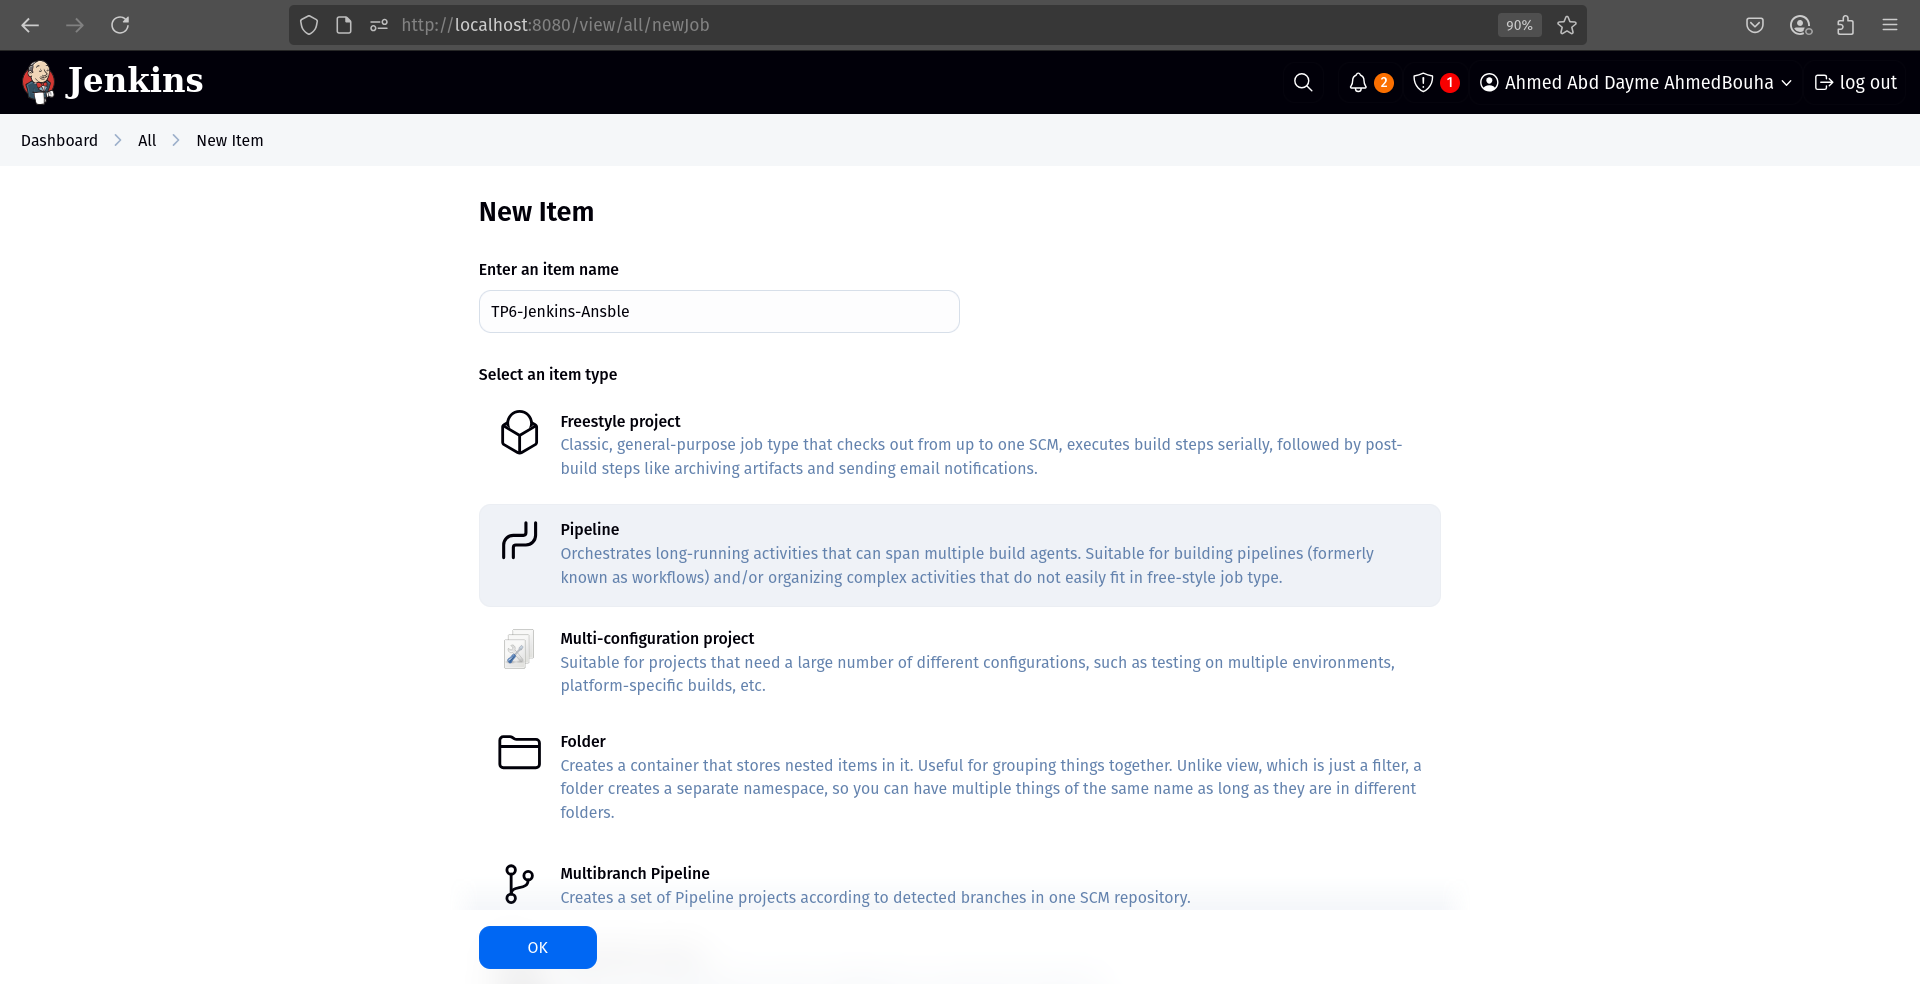
\includegraphics[width=0.8\textwidth]{images/jenkins_newitem.png}
    \caption{Création d'un nouveau job pipeline dans Jenkins}
    \label{fig:jenkins_newitem}
\end{figure}

\subsection{Configuration du pipeline}

Dans la page de configuration du pipeline, j'ai configuré les paramètres suivants :
\begin{enumerate}
    \item Dans la section "Pipeline", j'ai sélectionné "Pipeline script from SCM"
    \item Pour SCM, j'ai sélectionné "Git"
    \item Dans "Repository URL", j'ai entré l'URL de mon dépôt GitHub : \\
    \texttt{https://github.com/ahmedabddayme3752/dev\_ansible.git}
    \item Comme mon dépôt est public, je n'ai pas eu besoin d'ajouter d'identifiants
    \item Dans "Branch Specifier", j'ai laissé la valeur par défaut "\*/master"
    \item Dans "Script Path", j'ai vérifié que "Jenkinsfile" était bien spécifié
\end{enumerate}

\begin{figure}[h]
    \centering
    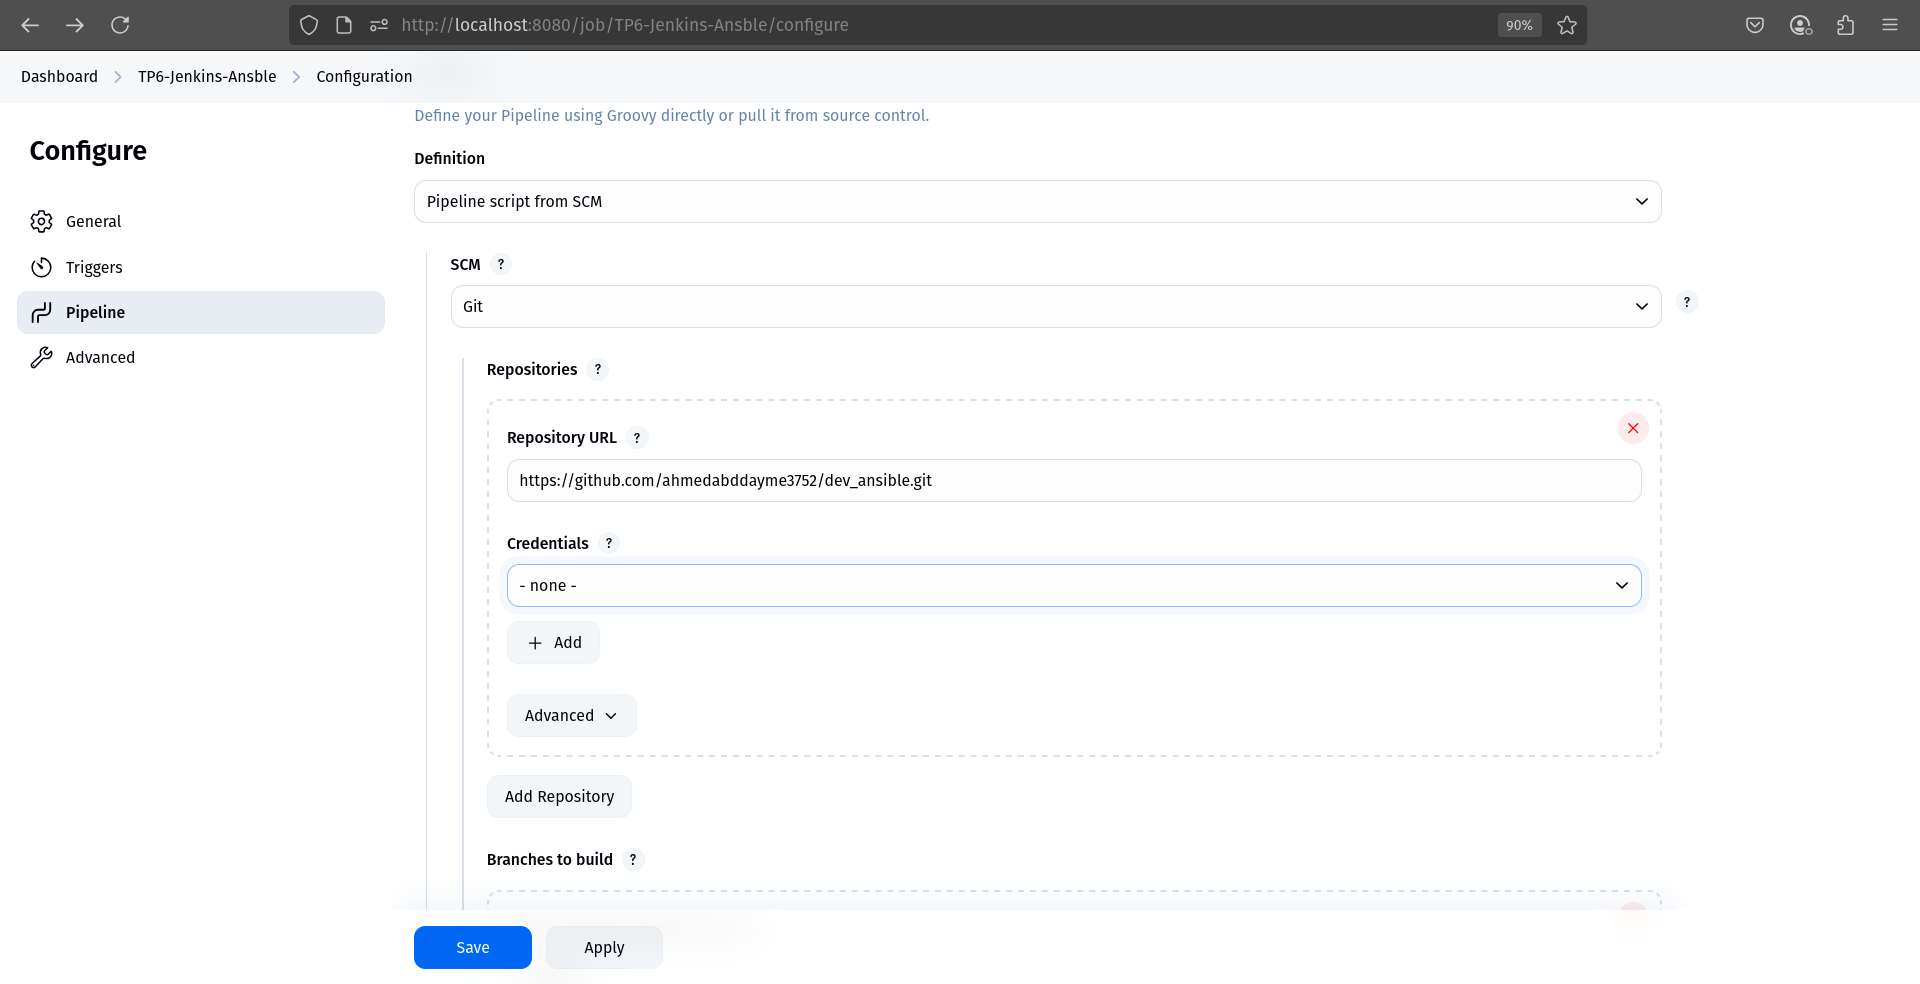
\includegraphics[width=0.8\textwidth]{images/jenkins_pipeline_config.png}
    \caption{Configuration du pipeline Jenkins}
    \label{fig:jenkins_pipeline_config}
\end{figure}

\subsection{Analyse du Jenkinsfile}

Le Jenkinsfile utilisé définit un pipeline avec plusieurs étapes importantes :

\begin{lstlisting}[language=groovy]
pipeline {
    agent any
    
    environment {
        ANSIBLE_INVENTORY = "${WORKSPACE}/inventory.ini"
        ANSIBLE_PLAYBOOK = "${WORKSPACE}/deploy.yml"
    }
    
    stages {
        stage('Checkout') {
            steps {
                // Checkout code from the GitHub repository
                checkout scm
            }
        }
        
        stage('Check Ansible') {
            steps {
                // Check if Ansible is installed
                sh '''
                    if command -v ansible &> /dev/null; then
                        echo "Ansible is already installed"
                        ansible --version
                    else
                        echo "Ansible is not installed. Please install it before running this pipeline."
                        exit 1
                    fi
                '''
            }
        }
        
        stage('Deploy with Ansible') {
            steps {
                // Run the Ansible playbook to deploy the application
                ansiblePlaybook(
                    playbook: "${ANSIBLE_PLAYBOOK}",
                    inventory: "${ANSIBLE_INVENTORY}",
                    colorized: true
                )
            }
        }
    }
}
\end{lstlisting}

Ce pipeline est composé de trois étapes principales :
\begin{enumerate}
    \item \textbf{Checkout} : Récupère le code source depuis le dépôt GitHub
    \item \textbf{Check Ansible} : Vérifie si Ansible est déjà installé
    \item \textbf{Deploy with Ansible} : Exécute le playbook Ansible pour déployer l'application
\end{enumerate}

\section{Configuration d'Ansible}
\subsection{Fichier d'inventaire}

Le fichier \texttt{inventory.ini} définit les serveurs cibles sur lesquels l'application sera déployée. Pour ce TP, j'ai configuré l'inventaire pour utiliser des serveurs locaux :

\begin{lstlisting}
[web]
localhost ansible_connection=local

[db]
# db1.example.com ansible_user=ubuntu
# db2.example.com ansible_user=ubuntu

# Variables that will be applied to all servers
[all:vars]
ansible_python_interpreter=/usr/bin/python3
\end{lstlisting}

Pour faciliter les tests sans avoir à configurer des serveurs distants, j'ai utilisé principalement la section \texttt{[local]} qui permet de déployer l'application sur la machine locale.

\subsection{Playbook Ansible}

Le playbook \texttt{deploy.yml} définit les tâches nécessaires pour déployer l'application :

\begin{lstlisting}[language=yaml]
---
- name: Test deployment 
  hosts: web
  become: no
  gather_facts: yes
  
  tasks:
    - name: Echo success message
      debug:
        msg: "This is a test deployment on {{ inventory_hostname }}"

    - name: Display ansible version
      debug:
        msg: "Ansible version: {{ ansible_version.full }}"

    - name: Create a test file
      file:
        path: /tmp/ansible_test.txt
        state: touch
        mode: '0644'

    - name: Write to test file
      copy:
        content: "Deployment test successful on {{ ansible_date_time.date }} at {{ ansible_date_time.time }}"
        dest: /tmp/ansible_test.txt

    - name: Show content of test file
      command: cat /tmp/ansible_test.txt
      register: file_content
      changed_when: false

    - name: Display file content
      debug:
        var: file_content.stdout_lines
\end{lstlisting}

Ce playbook effectue plusieurs opérations de test :
\begin{enumerate}
    \item Affiche un message de succès
    \item Affiche la version d'Ansible
    \item Crée un fichier de test dans /tmp
    \item Écrit un message de déploiement réussi dans le fichier
    \item Affiche le contenu du fichier
\end{enumerate}

\section{Exécution du pipeline}
\subsection{Lancement du build}

Après avoir configuré le pipeline, j'ai lancé manuellement le build en cliquant sur "Build Now" ou "Lancer un build" dans l'interface Jenkins.

\begin{figure}[h]
    \centering
    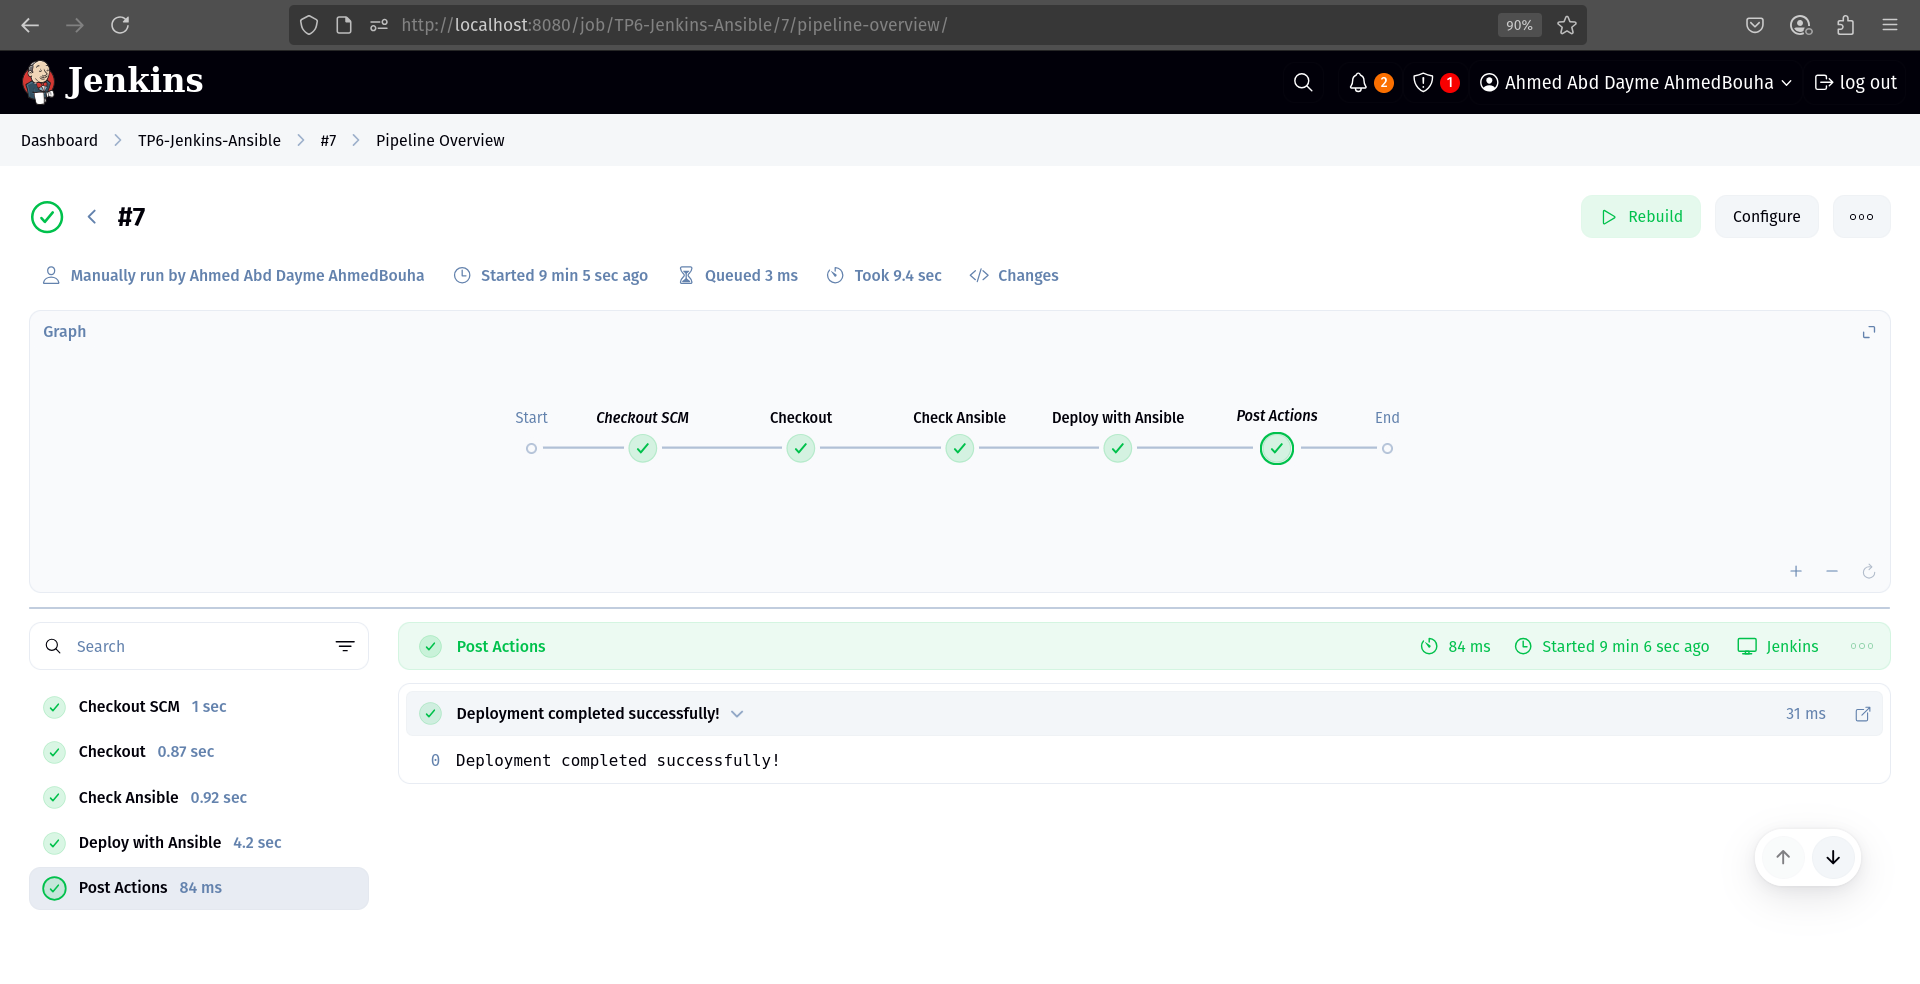
\includegraphics[width=0.8\textwidth]{images/jenkins_pipeline_dashboard.png}
    \caption{Tableau de bord du pipeline avant exécution}
    \label{fig:jenkins_pipeline_dashboard}
\end{figure}

\subsection{Suivi de l'exécution}

Pendant l'exécution du pipeline, j'ai pu suivre l'avancement des différentes étapes en temps réel grâce à la visualisation du pipeline et à la console de sortie.

\begin{figure}[h]
    \centering
    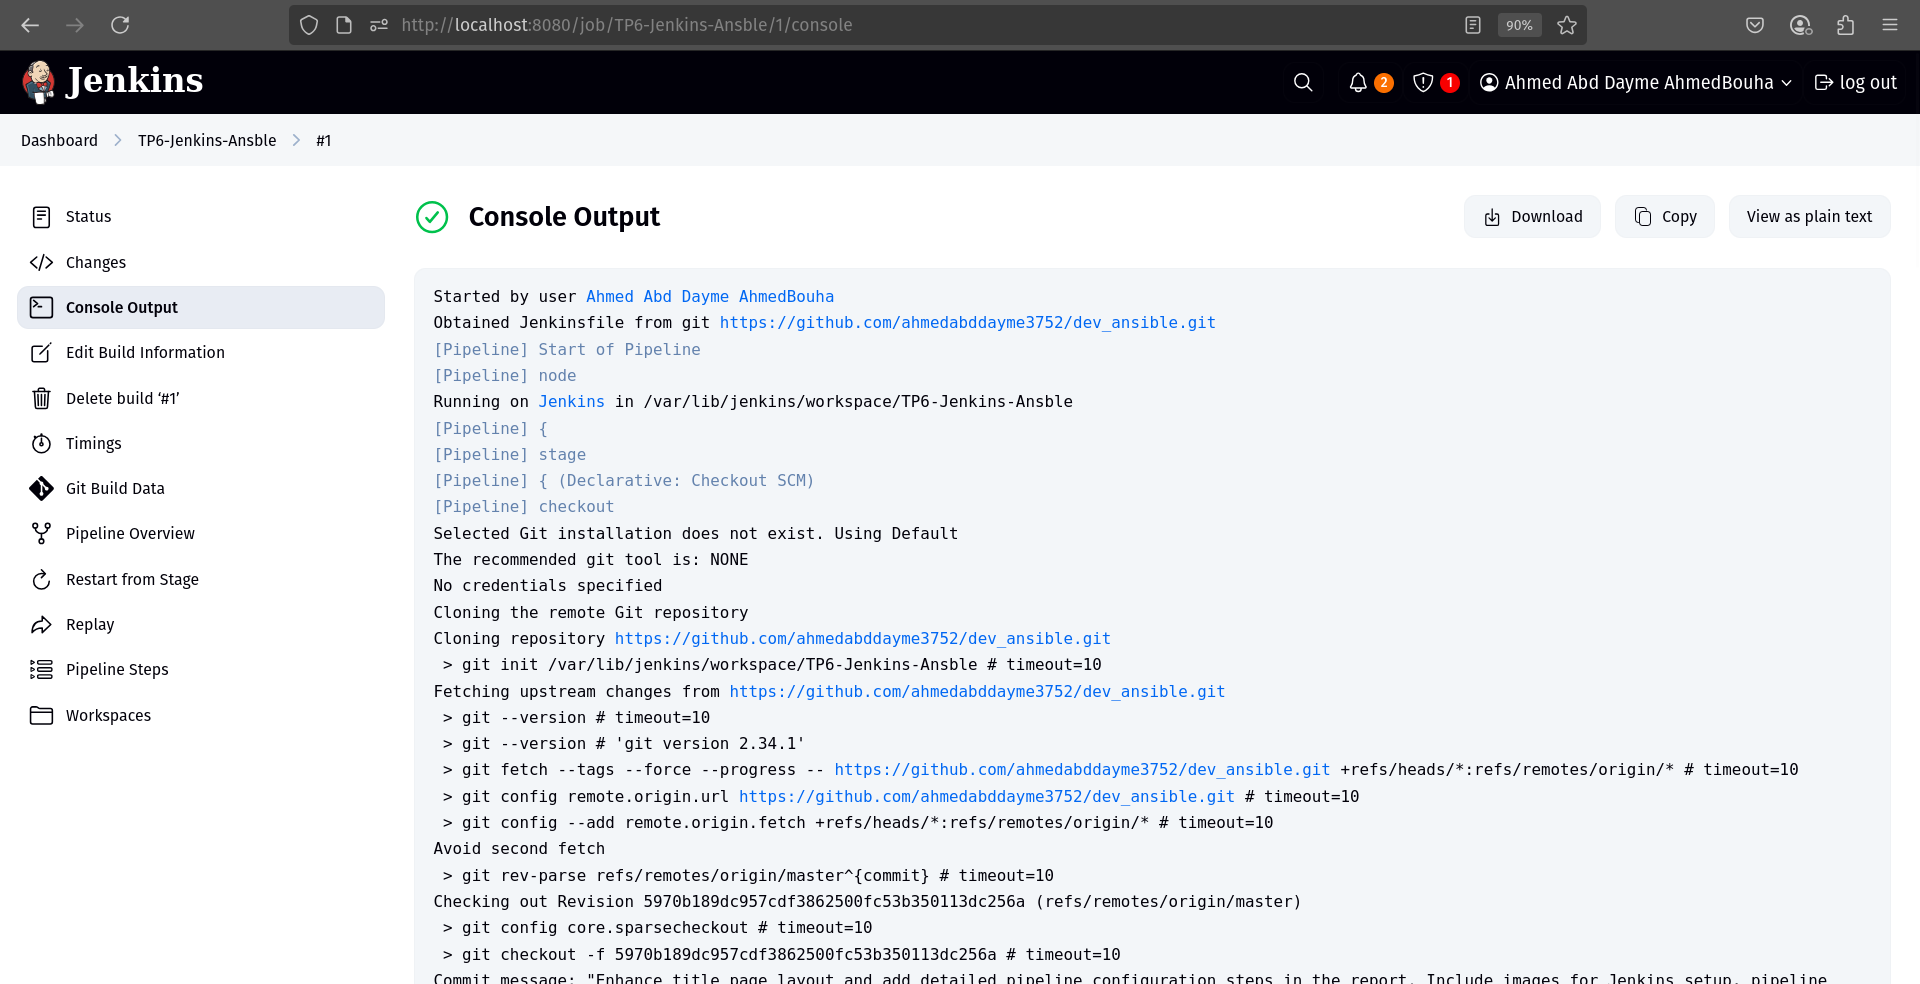
\includegraphics[width=0.8\textwidth]{images/jenkins_console_output.png}
    \caption{Console de sortie pendant l'exécution du pipeline}
    \label{fig:jenkins_console_output}
\end{figure}

\begin{figure}[h]
    \centering
    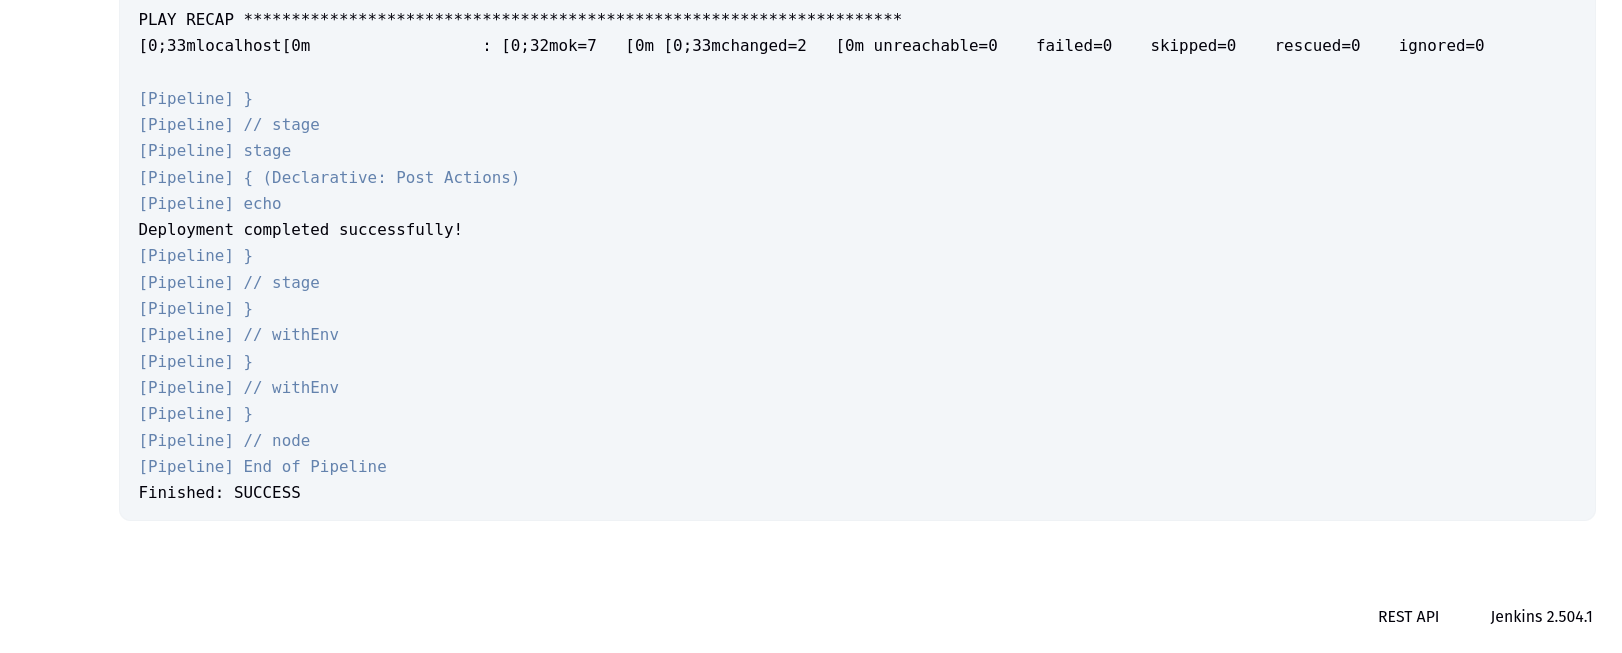
\includegraphics[width=0.8\textwidth]{images/jenkins_console_output_succes.png}
    \caption{Console de sortie montrant le succès de l'exécution}
    \label{fig:jenkins_console_output_succes}
\end{figure}

\subsection{Résultat du pipeline}

Une fois le pipeline terminé, j'ai pu observer le résultat global de l'exécution.

\begin{figure}[h]
    \centering
    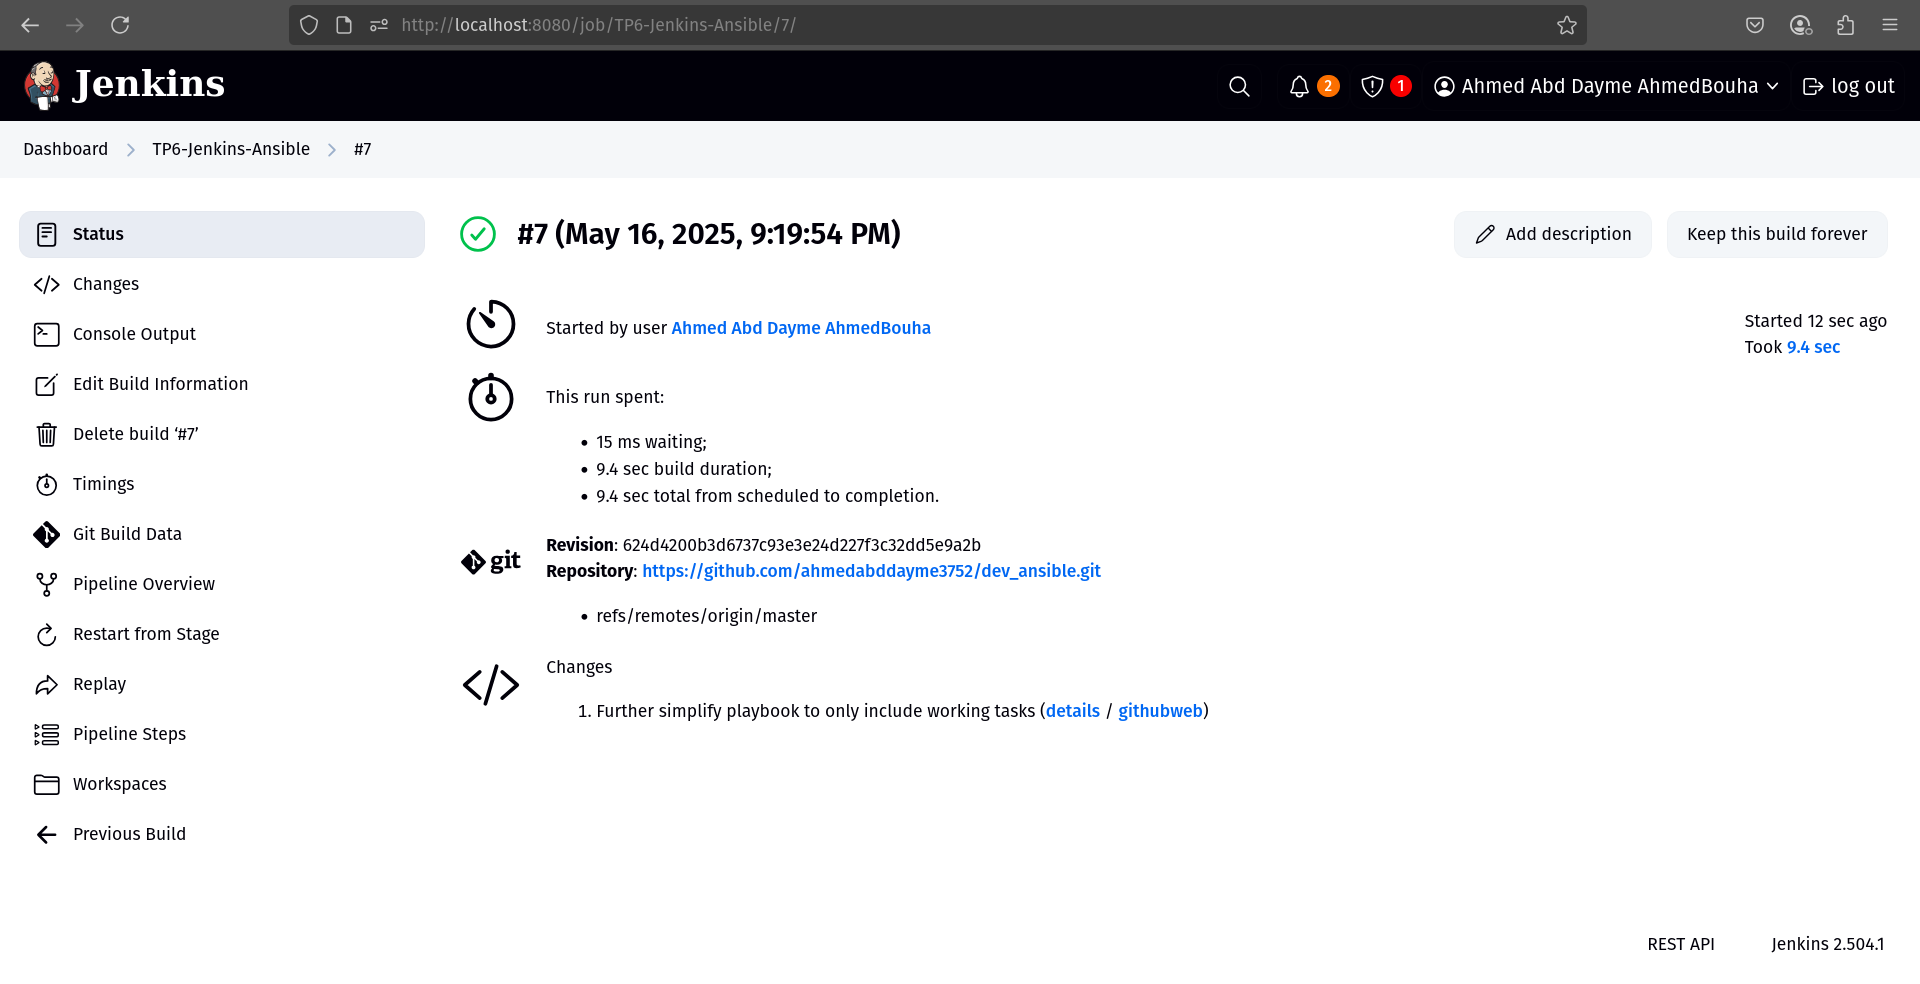
\includegraphics[width=0.8\textwidth]{images/jenkins_pipeline_simple.png}
    \caption{Pipeline Jenkins réussi avec playbook simplifié}
    \label{fig:jenkins_pipeline_simple}
\end{figure}

\section{Vérification du déploiement}
\subsection{Vérification des fichiers déployés}

Pour confirmer que le déploiement a bien fonctionné, j'ai vérifié la présence du fichier de test créé par Ansible :

\begin{lstlisting}[language=bash]
ls -la /tmp/ansible_test.txt
cat /tmp/ansible_test.txt
\end{lstlisting}

\begin{figure}[h]
    \centering
    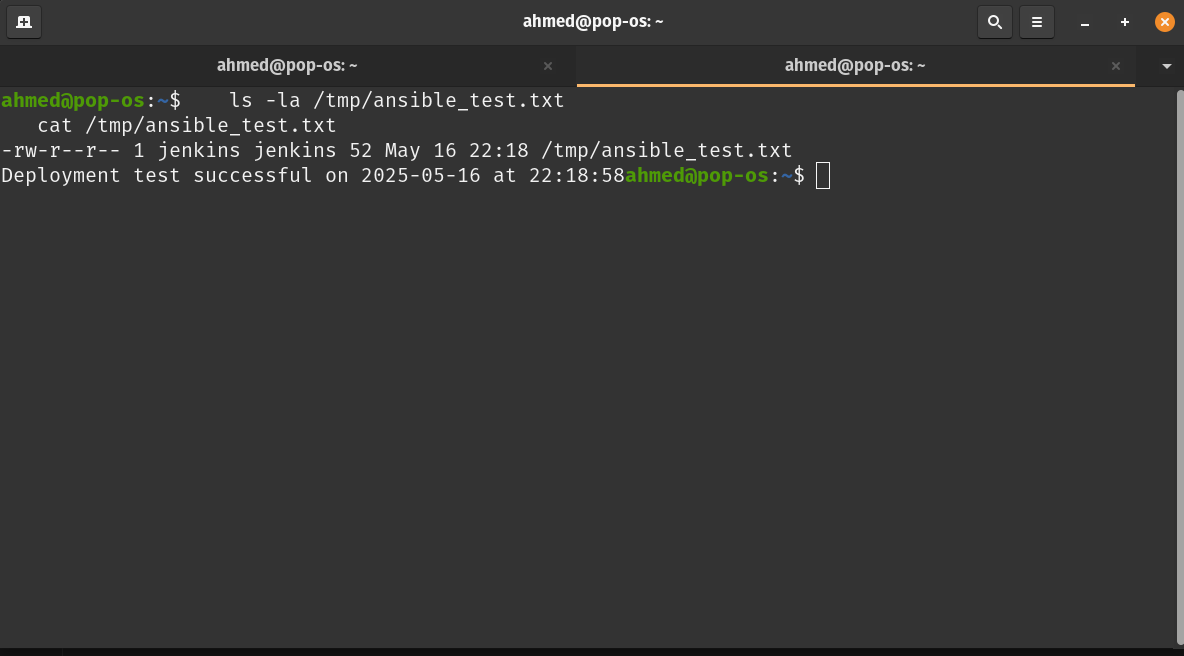
\includegraphics[width=0.8\textwidth]{images/deployed_files.png}
    \caption{Fichier de test déployé par Ansible}
    \label{fig:deployed_files}
\end{figure}

\section{Dépannage des problèmes rencontrés}
\subsection{Problème de permissions sudo}

Lors de la première exécution du pipeline, j'ai rencontré une erreur liée aux permissions sudo :

\begin{lstlisting}
+ sudo apt-get update
sudo: a terminal is required to read the password; either use the -S option to read from standard input or configure an askpass helper
sudo: a password is required
\end{lstlisting}

Ce problème s'est produit car Jenkins n'a pas le droit d'exécuter des commandes sudo sans mot de passe. Pour résoudre ce problème, j'ai modifié le Jenkinsfile pour éviter l'utilisation de sudo en remplaçant l'étape d'installation d'Ansible par une simple vérification :

\begin{lstlisting}[language=groovy]
stage('Check Ansible') {
    steps {
        // Check if Ansible is installed
        sh '''
            if command -v ansible &> /dev/null; then
                echo "Ansible is already installed"
                ansible --version
            else
                echo "Ansible is not installed. Please install it before running this pipeline."
                exit 1
            fi
        '''
    }
}
\end{lstlisting}

Cette modification présuppose qu'Ansible est déjà installé sur le serveur Jenkins, ce qui était le cas dans mon environnement. Dans un environnement de production, on pourrait envisager les solutions suivantes :

\begin{itemize}
    \item Préinstaller Ansible sur le serveur Jenkins
    \item Configurer sudo pour permettre à l'utilisateur Jenkins d'exécuter certaines commandes sans mot de passe
    \item Utiliser un conteneur Docker comme agent Jenkins avec Ansible préinstallé
\end{itemize}

\subsection{Simplification du playbook pour les tests}

Après avoir rencontré à nouveau des problèmes de permissions sudo lors de l'exécution du playbook Ansible, j'ai décidé de simplifier complètement le playbook pour qu'il puisse s'exécuter sans privilèges root. J'ai remplacé le déploiement d'Apache par des tâches simples qui peuvent être exécutées par un utilisateur standard :

\begin{lstlisting}[language=yaml]
---
- name: Test deployment 
  hosts: web
  become: no
  gather_facts: yes
  
  tasks:
    - name: Echo success message
      debug:
        msg: "This is a test deployment on {{ inventory_hostname }}"

    - name: Display ansible version
      debug:
        msg: "Ansible version: {{ ansible_version.full }}"

    - name: Create a test file
      file:
        path: /tmp/ansible_test.txt
        state: touch
        mode: '0644'

    - name: Write to test file
      copy:
        content: "Deployment test successful on {{ ansible_date_time.date }} at {{ ansible_date_time.time }}"
        dest: /tmp/ansible_test.txt

    - name: Show content of test file
      command: cat /tmp/ansible_test.txt
      register: file_content
      changed_when: false

    - name: Display file content
      debug:
        var: file_content.stdout_lines
\end{lstlisting}

Cette approche permet de démontrer le fonctionnement du pipeline CI/CD sans nécessiter de permissions spéciales. Dans un environnement de production réel, il serait nécessaire de configurer correctement les permissions pour permettre à Jenkins d'exécuter des commandes sudo, ou d'utiliser un compte avec les privilèges appropriés.

\begin{figure}[h]
    \centering
    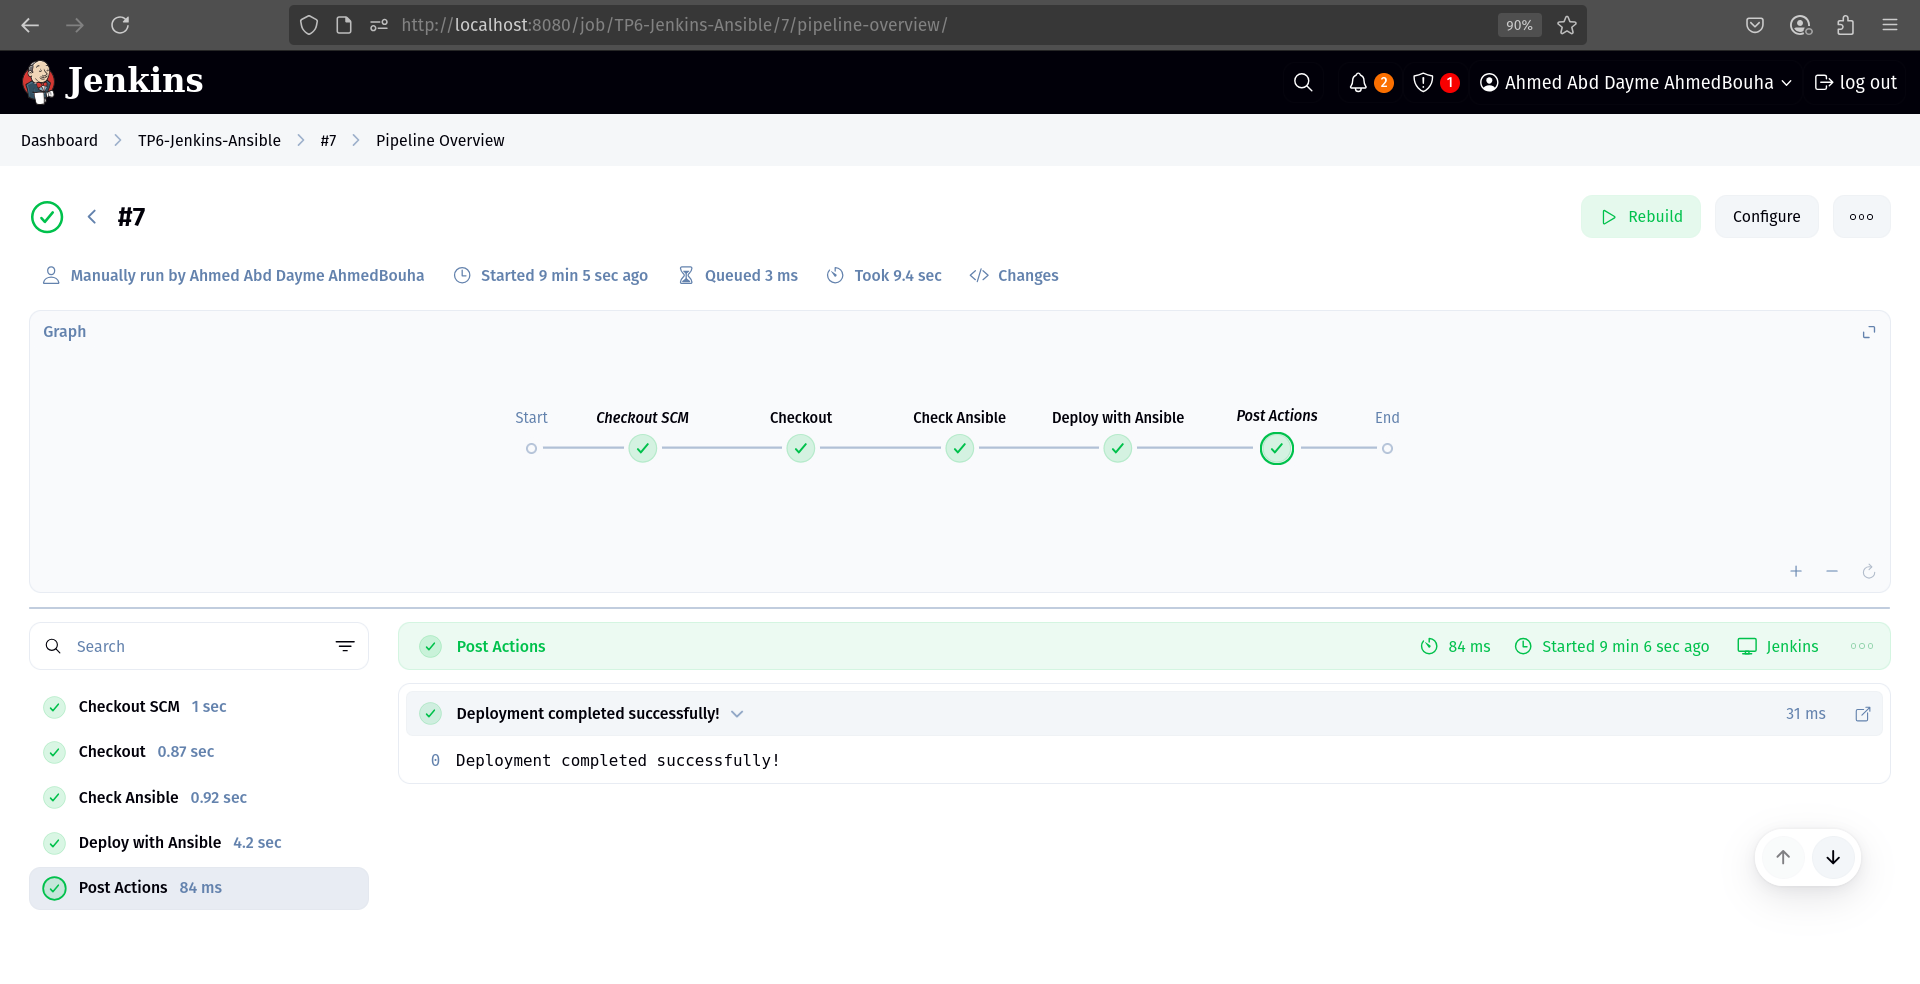
\includegraphics[width=0.8\textwidth]{images/jenkins_pipeline_success.png}
    \caption{Pipeline Jenkins après résolution des problèmes (exécution réussie)}
    \label{fig:jenkins_pipeline_success}
\end{figure}

\section{Conclusion personnelle}

Ce TP m'a permis de comprendre et d'appliquer les concepts d'intégration continue et de déploiement continu (CI/CD) en utilisant des outils modernes et très répandus dans l'industrie. J'ai pu constater l'efficacité d'une chaîne d'automatisation pour simplifier et fiabiliser le processus de déploiement logiciel.

La mise en place de l'intégration Jenkins-Ansible présente plusieurs avantages :
\begin{itemize}
    \item \textbf{Automatisation complète} du processus de déploiement, de l'extraction du code à sa mise en production
    \item \textbf{Reproductibilité} des déploiements grâce à la définition déclarative des tâches Ansible
    \item \textbf{Traçabilité} avec l'historique des déploiements et des logs conservés par Jenkins
\end{itemize}

Malgré les défis rencontrés avec les permissions sudo et la configuration des hôtes, j'ai réussi à mettre en place un pipeline fonctionnel qui démontre les principes de base de l'intégration continue. Les connaissances acquises pendant ce TP pourront être directement appliquées dans un contexte professionnel de DevOps.

\end{document} 